\section{Introduction}

\begin{figure*}[t]
\centering
\begin{subfigure}{0.5\textwidth}
  \centering
  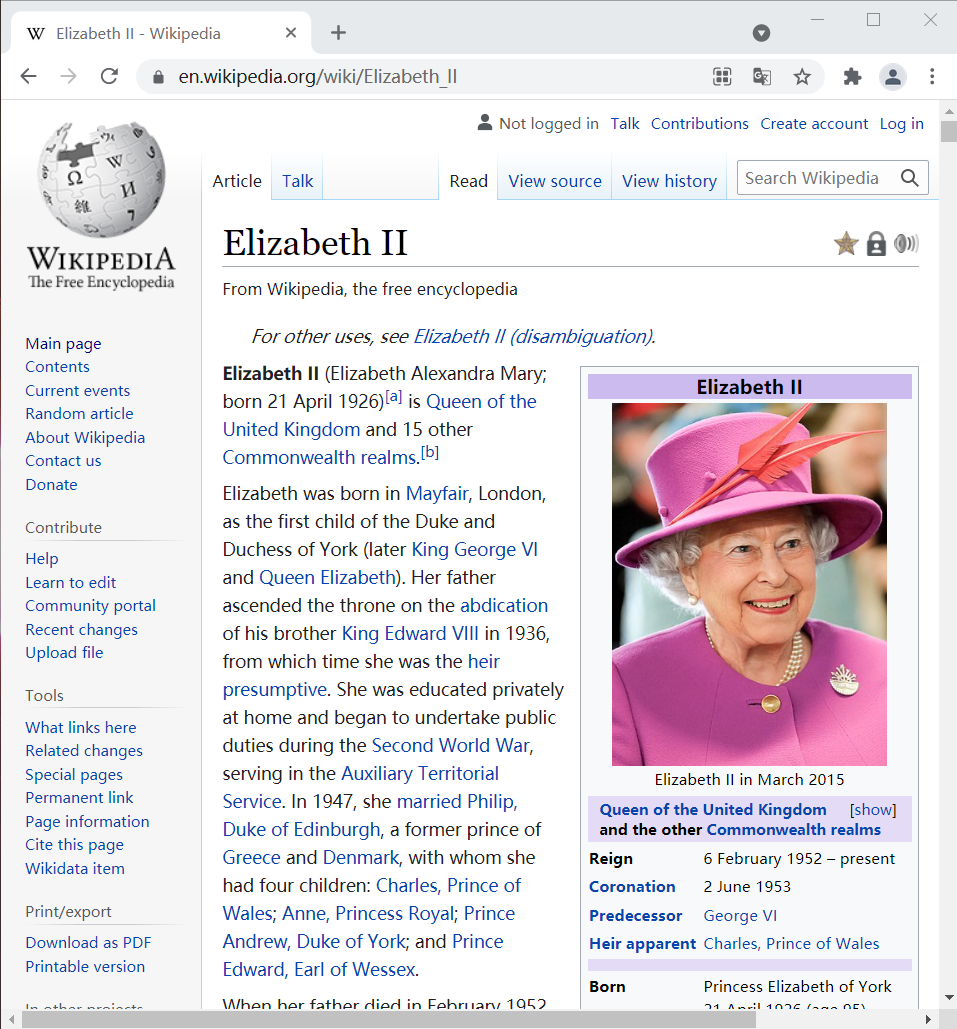
\includegraphics[width=1\textwidth]{intropage_pc}
  \caption{Chrome Explorer on PC}
  \label{intropage_pc}
\end{subfigure}%
\hspace{0.5in}
\begin{subfigure}{0.25\textwidth}
  \centering
  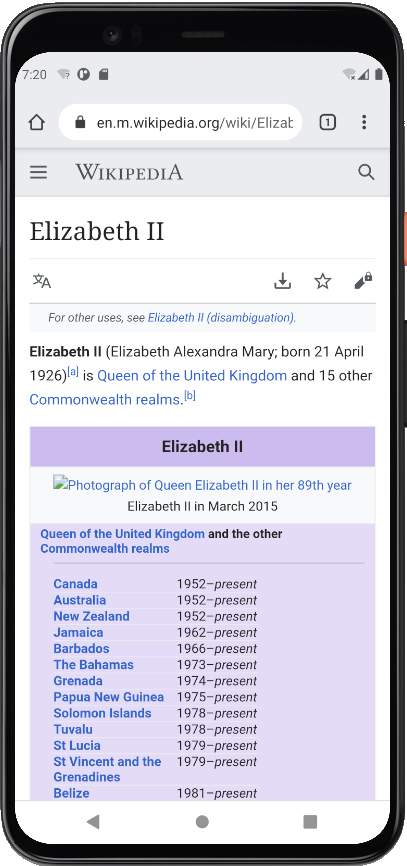
\includegraphics[width=1\textwidth]{intropage_phone}
  \caption{Android Phone}
  \label{intropage_phone}
\end{subfigure}
\caption{A sample web page rendered with different devices}
\label{intropage}
\end{figure*}

When reading texts, we frequently encounter unfamiliar entity names. For example, we may want to learn more about a person or a city mentioned in the article. Typically, we can obtain detailed information through search engines. However, this process can be inconvenient for readers, as it requires several steps: select the textual mention from the article, submit a query to the search engine, and then obtain relevant information from websites.

In such cases, we can have a better reading experience with hypertext links, which connect entities mentioned in the article to entries in a knowledge base. An important feature of Wikipedia is hypertext links. By assigning hyperlinks to the detected entity mentions in articles, users can easily access related information. However, not every detected entity mention needs to be linked. Excessive linking overwhelms the readers with unnecessary connections and can degrade the reading experience. For an overlinked article, the excessive amount of links makes it difficult for readers to identify the really helpful links. For each detected entity, to link or not to link naturally becomes a problem. Therefore, the quality of hyperlinks is our major concern.

Typically, the number of clicks a hyperlink receives indicates the link quality. A high-quality link should get regularly clicked by users, while an unnecessary link is rarely clicked. 
In fact, only around 4\% of all existing links on Wikipedia are clicked by visitors more frequently than 10 times within a month \cite{dimitrov2017makes}. Also, a previous study \cite{paranjape2016improving} states that 66\% links were not clicked even a single time in March 2015 and that most links were clicked very rarely. 

To better improve the reading experience, it is thus important to identify the frequently clicked links. In this paper, we study predicting the click popularity of hypertext links. Since the links on Wikipedia are manually created, we assume that all of the entity mentions have been correctly recognized, disambiguated, and linked. Our objective is to predict the most frequently clicked entities. Given that the click popularity of a hyperlink highly depends on the number of views the article receives, we eliminate the impact of page views by considering it as a ranking problem. To be specific, we rank these linked entities on a certain Wikipedia article according to their number of clicks.

To tackle the problem of click popularity prediction, previous works mainly focus on textual and graph-based features \cite{thruesen2016link, dimitrov2017makes}. However, they neglected that visual factors also have significant impact to the number of clicks on links. The article structure is an example: a large share of user clicks comes from links in the lead section or the infobox \cite{lamprecht2017structure}. Links in these two sections are more eye-catching and thus easier to get noticed by users.

In limited work that considered visual features \cite{dimitrov2016visual, dimitrov2017makes}, they render Html pages on PC under $1920 \times 1080$ resolution and then obtain the coordinate positions of hyperlinks as a type of feature. However, this approach has two drawbacks. First, the computation burden is heavy. The visual features cannot be obtained until the whole Html page has been completely rendered. Second, it is not reasonale to assume that all users to browse web pages exactly under the same setting. As is shown in Figure \ref{intropage}, even the same web page \footnote{https://en.wikipedia.org/wiki/Elizabeth\_II} can be rendered completely differently under different situations. Much more content can be rendered on PC than on Android Phone. Some link likes \emph{King Edward VIII} and \emph{heir presumptive} are placed in the middle part of the PC screen, but remains unspotted on Android Phone until users scroll down the explorer. Besides, the coordinate positions of these hyperlinks are also different. If people tend to click hyperlinks in the left part of the screen, the predicted result could be quite different under these two settings.

Therefore, visual features should be more general and independent of specific settings like devices and resolutions. In this work, we propose five visual features for ranking hypertext links, every of which does not require rendering web pages. They can be further combined with textual and graph-based features \cite{thruesen2016link, dimitrov2017makes} in a Learning to Rank algorithm for better ranking performance. To validate the effectiveness of visual features, we conduct controlled experiments with different sets of features. Moreover, we analyze the influence of each visual features through an ablation test.

To sum up, the main contributions of this paper are listed as the following:

\begin{itemize}

    \item First, we study hyperlink click popularity prediction and propose five visual features: \emph{section position}, \emph{distance to the nearest picture}, \emph{distance to the nearest subtitle}, \emph{distance to nearest table} and \emph{within table}. All these five features are independent of devices and resolutions and can be computed without rendering. Besides, our proposed visual features are orthogonal to all the other types of features, meaning that they can be combined with any other sets of features to improve accuracy for this task.

    \item Second, we validate the effectiveness of our proposed five visual features. We tested under ten different Wikipedia categories (People, Mass media, Culture, etc). According to the experimental results, the performance of the Learning to Rank algorithm can get improved after adding our visual features, which shows consistent improvement across different domains.
    
    \item Third, we compare our proposed visual feature with the previous ones that requires rendering \cite{dimitrov2017makes} under three most widely-used resolution settings (1366×768, 1536×864 and 1920×1080). Our proposed visual features can achieve higher performance, which suggests that the proposed render-free visual features can adapt better to practical scenarios with various resolution settings.

    \item Fourth, we further conduct ablation tests to quantitively analyze the influence of all these five visual features. The results indicate that every visual feature we proposed is helpful in this task. Besides, \emph{section position} and \emph{within table} are relatively more important.

\end{itemize}
